
% !TEX encoding = UTF-8 Unicode

\documentclass[twocolumn,10pt,a4j]{ltjsarticle}
\usepackage{kougai}
\usepackage{siunitx}

\title{音響プロジェクターのための音場測定}
\author{2032137 松村 泰河  指導教員 須田 宇宙 准教授}
\date{}

\begin{document}

\maketitle


\section{はじめに}
%背景
現代では音響分野のオーディオ技術が著しく成長している.
例を挙げると,5.1chや7.1ch等の多チャンネルでの視聴が可能となっているHD-DVD・Blu-ray Discが登場し,自宅で映画鑑賞などが可能となるホームシアターの普及がある.
音響技術の発展により,音波を聴取者の位置に向けることで臨場感を持たせることが可能となっている.

%問題点
5.1ch,7.1ch等のサラウンド環境は,聴取者が最適な位置にいる場合のみを想定したスピーカーの配置が研究されている\cite{kurosumi1994}.
そのため,位置や体勢を変えるなど,複数人での利用は想定されていない.
また,サラウンド環境では映像内の話者の位置と実際の音の位置に差がある.
その問題を改善することを目的としてオーセンサラウンドが開発された\cite{authensurround}.
オーセンサラウンドは,ディスプレイから出る音声に音像定位を利用した信号を加えることで,映像内の話者の位置と実際の音の位置の差を無くして臨場感を持たせることができる音響機器である.
しかし,オーセンサラウンドは大画面には対応していないという問題点がある.
また,SONY社に360 Reality Audioという技術がある\cite{360RealityAudio}.


%提案
これらの問題点を解決するために,聴取者が最適な位置にいなくてもスクリーン上の話者の口元等に仮想音源を置き,臨場感を持たせる機器の開発を考案する.
%目的
この機器を音響プロジェクターと呼び,音響プロジェクターの実現に向けて,音場を測定することを目的とする.

\section{音響プロジェクターの構想}
図\ref{fig:音響プロジェクター}は音響プロジェクターを用いた際の使用イメージである.
鋭い指向性の音波を画面上の対象の話者の口元に当て,その位置から音が広がるような仕組みである.
理想状態では,スクリーン上の仮想音源から音が広がっているような感覚となっているため,聴取者は位置を縛られず,複数人での聴取が可能となる.

本研究の最終的な目的としては,鋭い指向性の音波を画面に反射させることで,聴取者の位置によらず大画面でも臨場感のある音場環境を作ることである.

\vspace{1ex}
\begin{figure}[h]
\begin{center}
 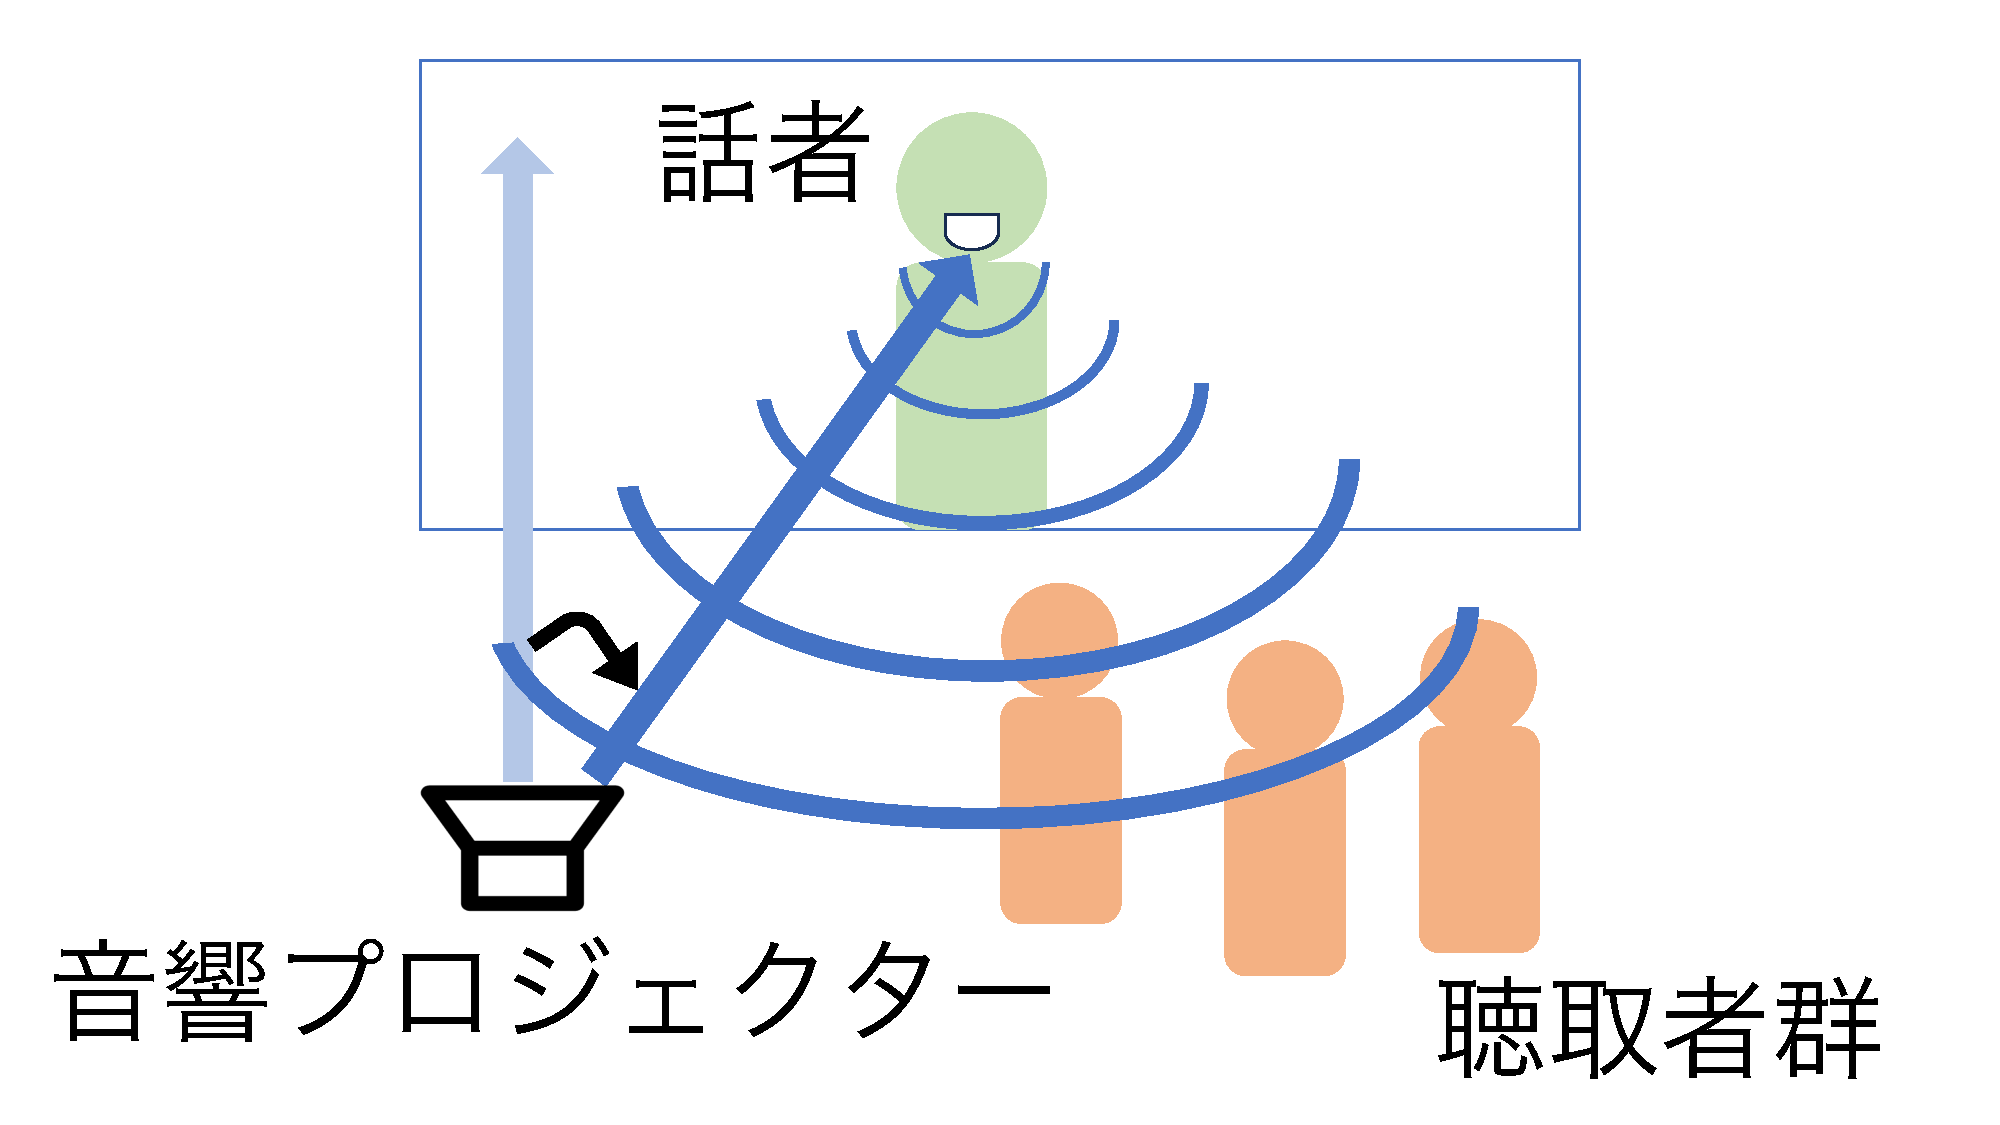
\includegraphics[clip,width=70mm,height=40mm]{onkyouP.pdf}
\end{center}
 \caption{音響プロジェクターの使用イメージ}
 \label{fig:音響プロジェクター}
\end{figure}


\section{音響プロジェクターの実現のための音場測定}

一般的に鋭い指向性を作る方法として,音響ホーンやパラメトリックスピーカーが知られている.
そこで,本研究ではこれらの機器を使用し,鋭い指向性を持つ音波をスクリーンにあてて,音場を測定する.

音響プロジェクターの実際の使用を想定して音場の測定を行なった.
音場測定は,まず,指向性スピーカーを用いて鋭い指向性を持つ音波を生成し,スクリーンに向けて音波を反射させる.
次に,反射後の音波をオシロスコープにつなげたマイクで音圧の測定を行う.
本研究の実験では,スクリーンと指向性スピーカーの距離と等しい距離にマイクを置いて,マイクを$\ang{10}$から$\ang{170}$の位置に$\ang{5}$ずつ移動させることで,各角度の音圧を測定し,音場を可視化している.
また,指向性スピーカーは$\ang{0}$・$\ang{15}$・$\ang{30}$に移動させて,音源の角度による音場を計測することで各角度での比較を行えるようにしている.


例として,図\ref{fig:結果}にスピーカーアレイで8000Hzの周波数を出し,音源は$\ang{90}$の位置と$\ang{75}$の位置に配置して音波を出している.
この図から,音源が$\ang{90}$のときは入射角と反射角が$\ang{0}$であり,$\ang{90}$付近の音圧が高くなっている.
また,音源が$\ang{75}$のときは入射角と反射角が$\ang{15}$であり,$\ang{105}$付近の音圧が高くなっている.
この結果から音波の大部分では幾何光学的に反射していることがわかる.


%\begin{equation}
%\scalebox{1.2}{$\displaystyle
%\label{eqn:ookisa}
%D=\left|\frac{P}{P_{\theta=0}} \right| =\left|\frac{\pi^2}{\pi^2-\left(\frac{kl\sin\theta}{2} \right)^2}\frac{\sin\left(\frac{kl\sin\theta}{2} \right)}{\left(\frac{kl\sin\theta}{2} \right)}\right|
%$}
%\end{equation}


\vspace{1ex}
\begin{figure}[h]
\begin{center}
 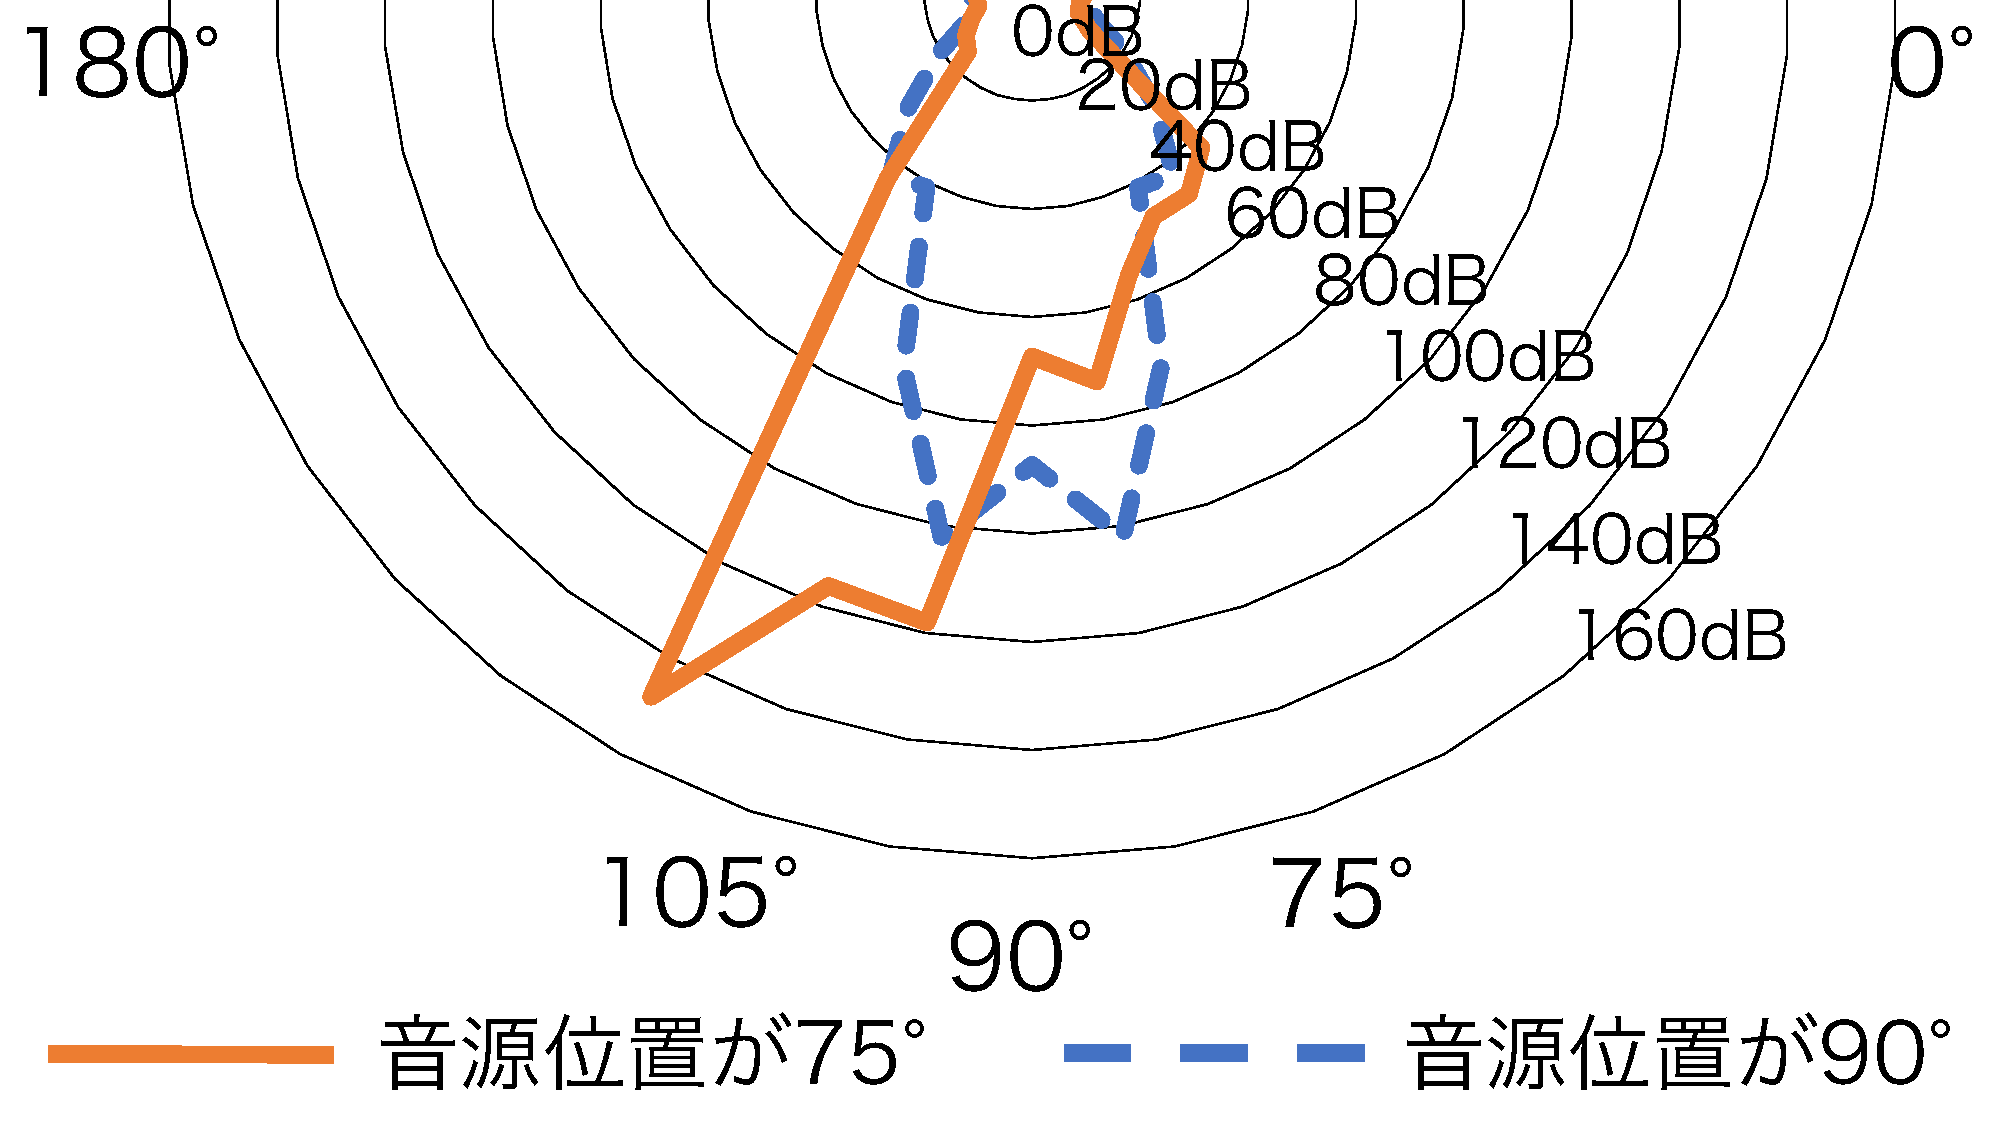
\includegraphics[clip,width=70mm,height=40mm]{keltuka.pdf}
\end{center}
 \caption{実験結果}
 \label{fig:結果}
\end{figure}

例として,図\ref{fig:結果}にスピーカーアレイで8000Hzの周波数を出し,音源は$\ang{90}$の位置と$\ang{75}$の位置に配置して音波を出している.
この図から,音源が$\ang{90}$のときは入射角と反射角が$\ang{0}$であり,$\ang{90}$付近の音圧が高くなっている.
また,音源が$\ang{75}$のときは入射角と反射角が$\ang{15}$であり,$\ang{105}$付近の音圧が高くなっている.
この結果から音波の大部分では幾何光学的に反射していることがわかる.

\vspace{1ex}
\begin{figure}[h]
\begin{center}
 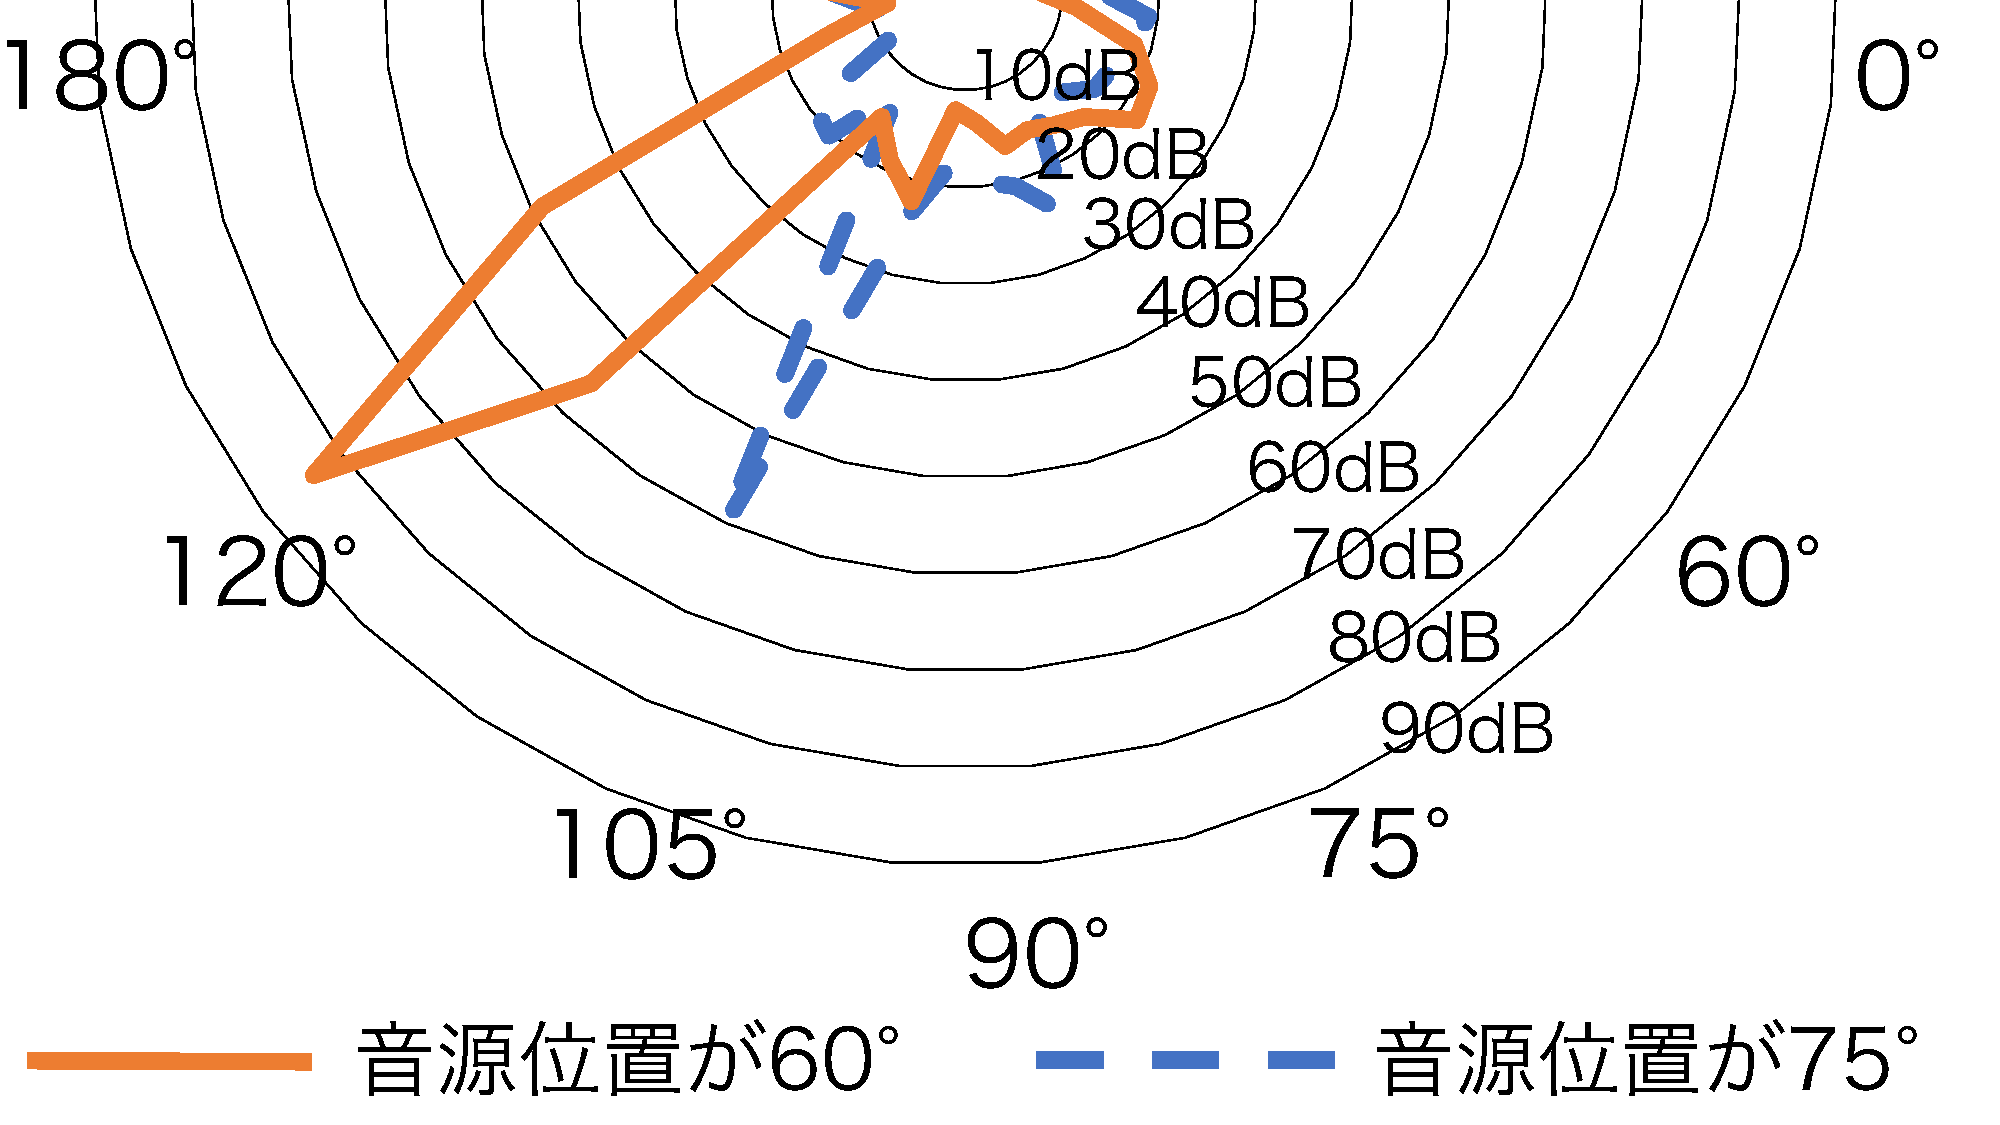
\includegraphics[clip,width=70mm,height=40mm]{keltuka2.pdf}
\end{center}
 \caption{実験結果}
 \label{fig:結果}
\end{figure}

例として,図\ref{fig:結果}にスピーカーアレイで8000Hzの周波数を出し,音源は$\ang{90}$の位置と$\ang{75}$の位置に配置して音波を出している.
この図から,音源が$\ang{90}$のときは入射角と反射角が$\ang{0}$であり,$\ang{90}$付近の音圧が高くなっている.
また,音源が$\ang{75}$のときは入射角と反射角が$\ang{15}$であり,$\ang{105}$付近の音圧が高くなっている.
この結果から音波の大部分では幾何光学的に反射していることがわかる.

\vspace{1ex}
\begin{figure}[h]
\begin{center}
 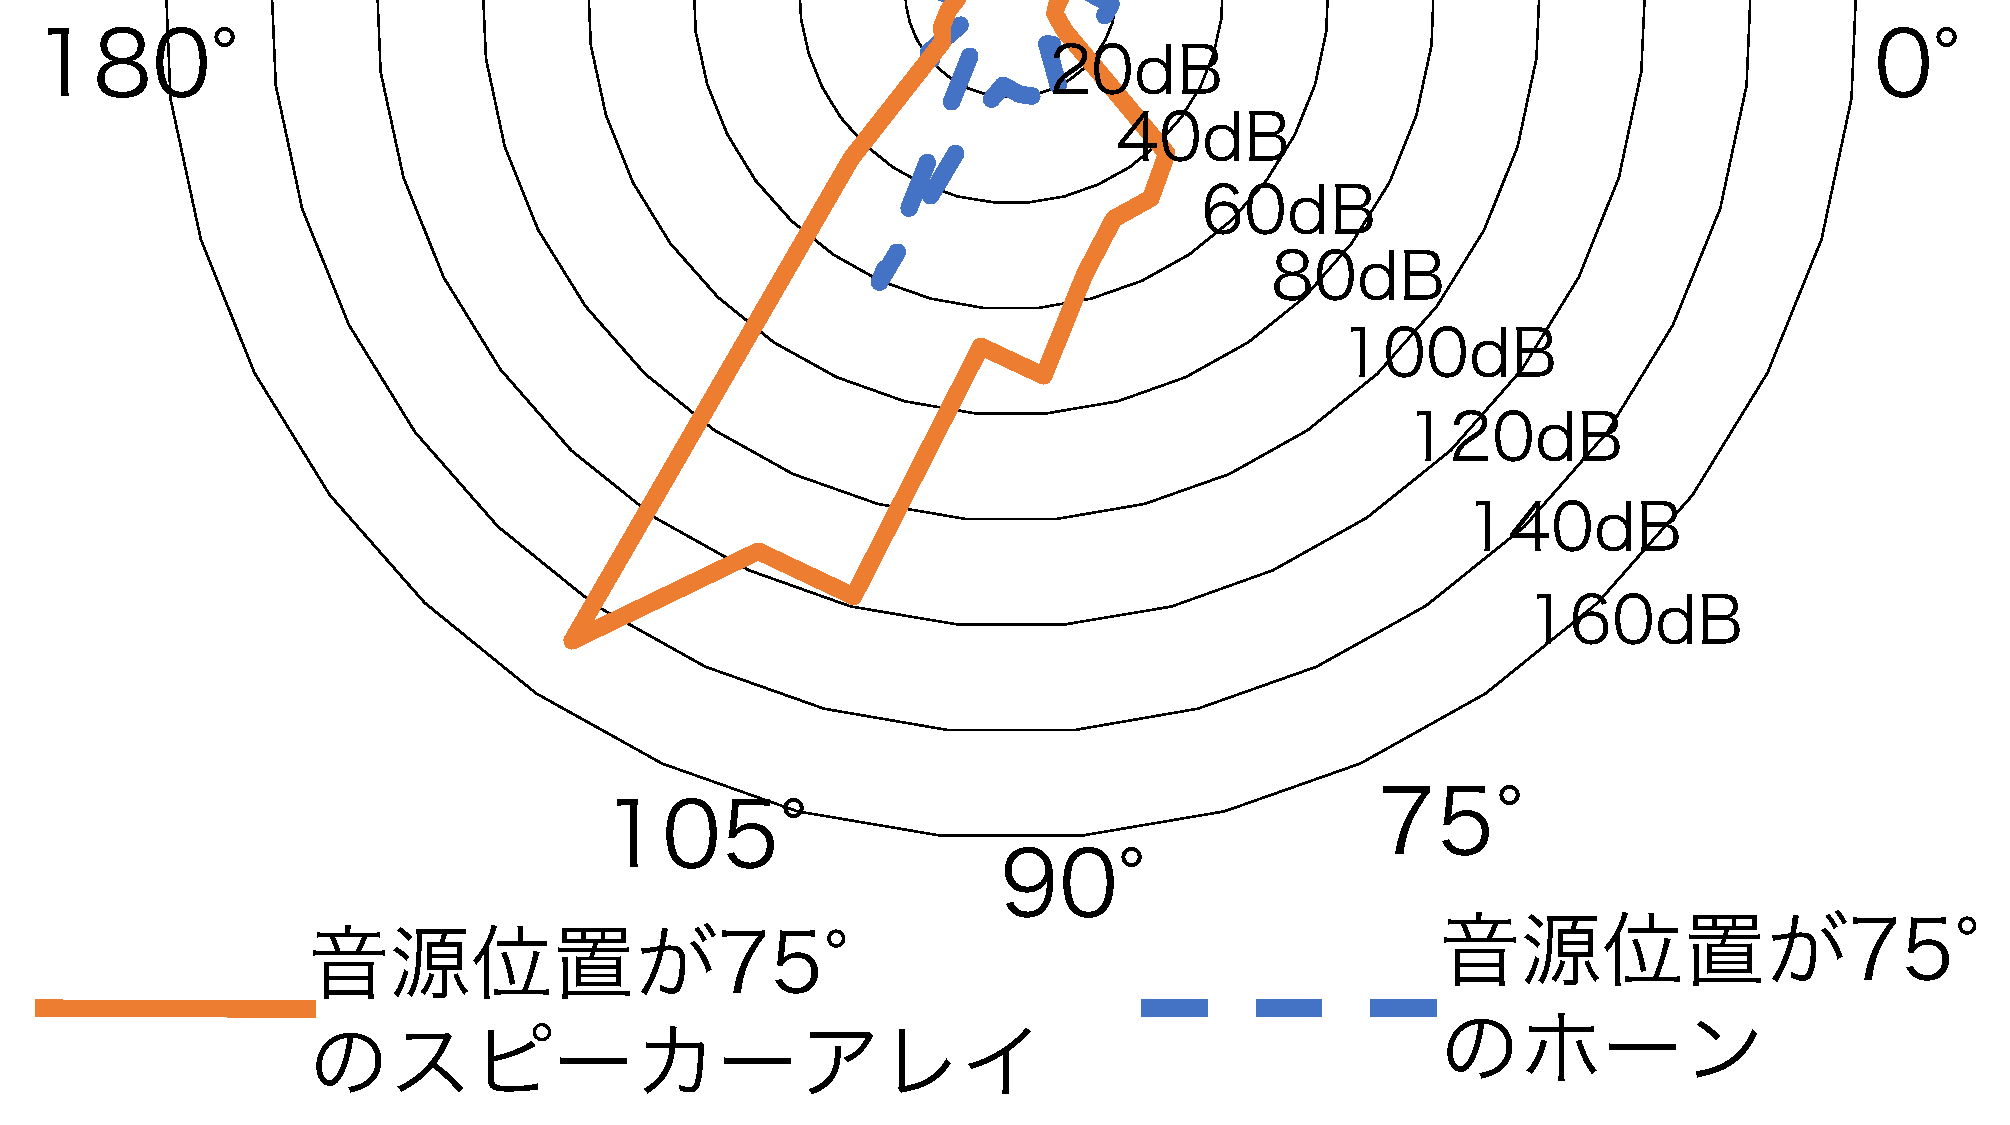
\includegraphics[clip,width=70mm,height=40mm]{keltuka3.pdf}
\end{center}
 \caption{実験結果}
 \label{fig:結果}
\end{figure}



\vspace{1ex}
\section{おわりに}
本研究では,鋭い指向性を持つ音波をスクリーンに反射させて音場を測定した.
そこで音波は幾何光学的に反射してしまうことが分かった.
この測定結果を活用して音響プロジェクターの実現を目指していく.

\begin{thebibliography}{99}
\bibitem{kurosumi1994} 黒住幸一: "放送におけるメルチチャネルステレオ音声方式'',日本音響学会誌,50巻11号 (1994) ,pp.915−920, 2023/7/7参照
\bibitem{authensurround} NEC Lavie: "https://support.nec-lavie.jp/product/pc/200509/common/function/sound/authensurround/index.html", 2023/7/18参照
\bibitem{360RealityAudio} 360 Reality Audio: "https://www.sony.jp/headphone/special/360\_Reality\_Audio/", 2023/12/24参照

\end{thebibliography}


\end{document}
